% Beamer template
% Author: Ozgur Taylan TURAN
% Delft University of Technology

\documentclass[aspectratio=169]{beamer}
% PACKAGES
\usepackage[english]{babel}
\usepackage{graphicx}
\usepackage{animate}
%\usepackage{calc}
\usepackage{calligra}
\usepackage[absolute,overlay]{textpos}
\usepackage[T1]{fontenc}
%\usefonttheme{serif}
\usefonttheme{professionalfonts}
\usepackage{amsmath}
\usepackage{palatino}
\usepackage{mathpazo}
\usepackage{graphicx}
%\usepackage{subfig}
\usepackage{tikz}
\usetikzlibrary{shapes,arrows}
\usepackage{xcolor}
\usepackage[T1]{fontenc}
%\usefonttheme{serif}
%\usepackage{titling}
\usepackage{graphicx}
%\usepackage{subfig}
%\usepackage{tikz}
%\usetikzlibrary{shapes,arrows}
\usepackage{mathtools}
\usepackage{cancel}
% CUSTOM PACKAGES
\usepackage{/home/taylanot/texmf/tex/beamerthemetot}
\input{/home/taylanot/texmf/presentation/tune.tex}

 % COVER PAGE INFO   
\newcommand{\mytitle}{\color{White}\huge{\textbf{Coffee Talk \#5}}}
\newcommand{\mysubtitle}{\color{Pink}\Large{\textbf{Gradient Descent on Neural Networks Typically Occurs at the Edge of Stability}}}
\newcommand{\myauthor}{\color{White}\textcalligra{\LARGE Ozgur Taylan Turan}}
\newcommand{\authorlabel}{\small O.T. Turan}
\author{\authorlabel}


\begin{document}
% COVER PAGE

{
\def\beamer@entrycode{\vspace*{-\headheight}}
\setbeamertemplate{frametitle}[default][center]
\setbeamertemplate{navigation symbols}{}
\usebackgroundtemplate{
\includegraphics[width=\paperwidth,height=\paperheight]{cover/coverart.pdf}}

\begin{frame}[plain] 

\begin{minipage}{\textwidth}
	\centering{\mytitle} \\
	%\vspace{1cm}
	%\centering{\mysubtitle} \\
	\vspace{1cm}
	\centering{\color{White}November 15, 2021} \\
	\vspace{1cm}
	\centering{\myauthor}\\
\end{minipage}
\end{frame}
}


\begin{frame}
	\centering
	\mysubtitle\cite{Cohen2021}
\end{frame}

\begin{frame}{Why This Paper?}
	\centering
	\begin{minipage}{0.8\textwidth}
			\centering
			 Interesting empirical result on gradient descent...
	\end{minipage}
\end{frame}

\begin{frame}{Stability of Gradient Descent}
	\begin{minipage}{0.5\textwidth}
    \centering
    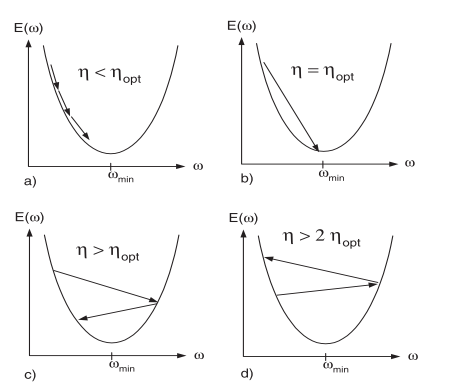
\includegraphics[width=0.9\textwidth]{Figures/GD.png}\cite{Orr1998}
	\end{minipage}%
	\begin{minipage}{0.5\textwidth}
    \begin{itemize}
      \item \textbf{Quadratic} Objective: $\text{E}(\omega)$
      \item $\omega_{t+1} = \omega_{t} - \eta E^\prime(\omega)$
      \item Learning Rate: $\eta$
      \item $\eta_{opt}=(E^{\prime\prime}(\omega))^{-1}$ inverse of Hessian
      \item If $\eta>2\eta_{opt}\quad\to$ \color{Pink}{Divergence}
    \end{itemize}
	\end{minipage}
\end{frame}

\begin{frame}{Gradient Descent on Neural Networks}
	\begin{minipage}{0.5\textwidth}
    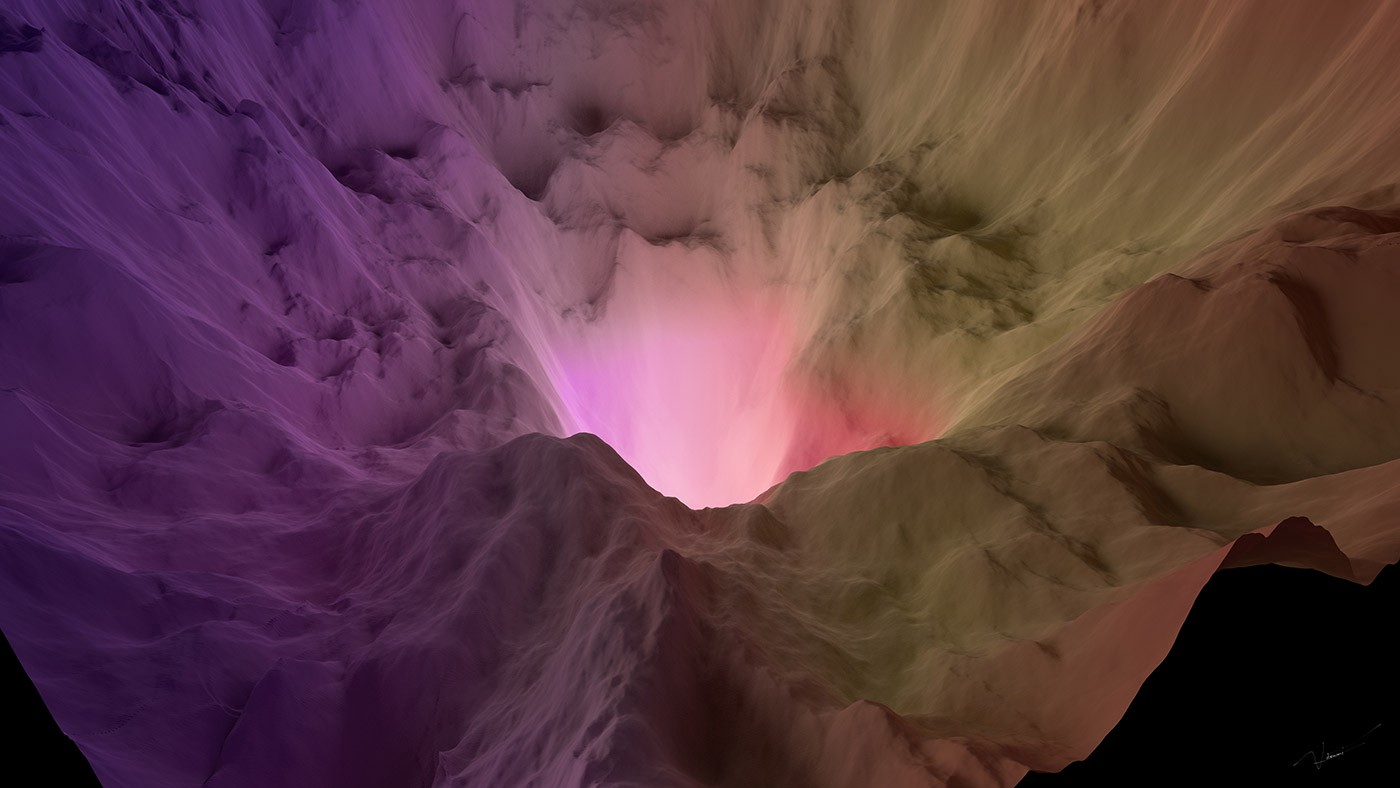
\includegraphics[width=\textwidth]{Figures/loss.jpeg}
    \center
    \color{Pink}https://losslandscape.com
	\end{minipage}%
	\begin{minipage}{0.5\textwidth}
    \begin{itemize}
      \item Losses ($\mathcal{L}(\omega)$) are not globally quadratic!
      \item But, second order Taylor expansion around any point in parameter space is Quadratic! 
      \item Then, if $\mathbf{H}>\frac{2}{\eta}\quad\to$ \color{Pink} Divergence
      \item \color{Black}Hessian largest eigenvalue = Sharpness
    \end{itemize}
	\end{minipage}
\end{frame}

\begin{frame}{Progressive Sharpening}
	\begin{minipage}{\textwidth}
    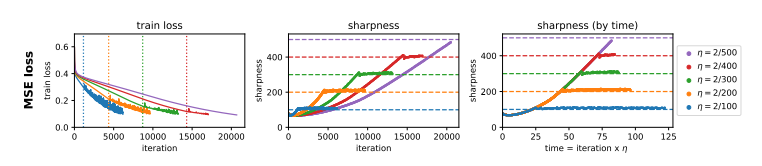
\includegraphics[width=\textwidth]{Figures/prog_sharp.png}
	\end{minipage}
	\begin{minipage}{\textwidth}
    \begin{itemize}
      \item Full-batch, vanilla-GD
      \item CIFAR-10/subset of 5000 examples
      \item Fully-connected/two-layer/200-width/tanh/stop-$99\%$ acc.
    \end{itemize}
	\end{minipage}
\end{frame}

\begin{frame}{Furthermore}
	\begin{minipage}{\textwidth}
    \begin{itemize}
      \item <1> Effect of width? \color{Pink} Lesser degree\color{Black}
      \item <2> Other Losses? \color{Pink}Different behaviour\color{Black}
      \item <3> Other experiments? \color{Pink}Changing arch.+tasks\color{Black}
    \end{itemize}
	\end{minipage}
  \begin{minipage}{\textwidth}
    \centering
    \includegraphics<1>[width=0.8\textwidth]{Figures/width.png}
    \includegraphics<2>[width=0.8\textwidth]{Figures/cross_entropy.png}
  \end{minipage}
\end{frame}

\begin{frame}{Conclusions}
	\begin{minipage}{\textwidth}
    \begin{itemize}
      \item Training loss decrease is non-monotonic
      \item \color{Pink} \textit{L}-smoothness \color{Black} assumption might be in jeopardy... (convergence analysis)
      \item Edge of Stability is inherently non-quadratic
    \end{itemize}
	\end{minipage}
\end{frame}



\end{document}

